% !TeX root = ../main.tex

\chapter{Related work}  \label{chapter:relatedwork}

This chapter presents existing deep learning approaches that have addressed the issue of future frame prediction. These are grouped into three sections depending on the model implementation, namely neural networks, recurrent networks and adversarial networks. The strength, weaknesses and design decisions of these models are briefly discussed, together with a short analysis of the achieved outcomes. Further, it is highlighted how these approaches have influenced the architecture of our final model that is used throughout the evaluation in Chapter \ref{chapter:evaluation}. Aside from that, their results form the baseline in the assessment of our model.


\section{Neural Network Approach}

First approaches to predict a future images in an image sequence have been done in \parencite{ann} and its follow-up publication \parencite{ann2}. Probably due to the lower computational power and the weak development of CNNs at that time, they tried to perform single frame prediction based on an artificial neural network. Several preprocessing steps have been performed in order to train such a model using image data. Firstly, they have split the images by the R, G and B color channels into three parts. Next, the dimension of data has been reduced from the order of $10^4$ to $100$ in each case using techniques like \textit{principle component analysis} (PCA)\footnote{PCA: Technique to reduce the data dimensionality by mapping it into its eigenspace.}. The final training and inference has then been accomplished on three seperate neural neutworks of the same architecture for each color channel. After each prediction, the PCA process is inverted to obtain the initial dimensionaly, as well as all three outputs are combined to obtain the final image.

\begin{figure}[htb]
\centering
\begin{subfigure}{0.5\textwidth}
  \centering
  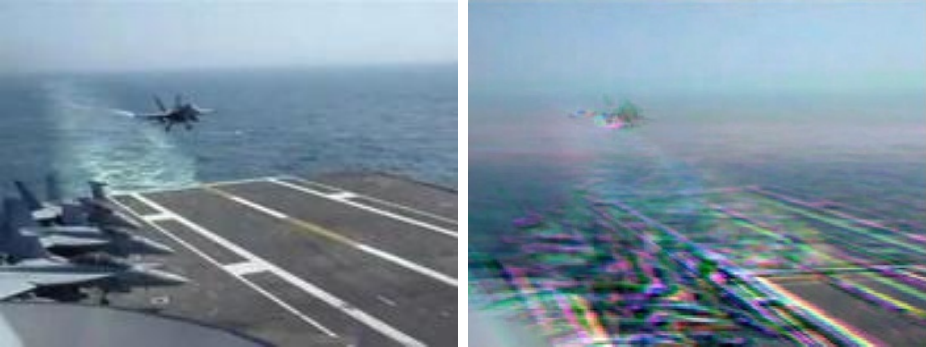
\includegraphics[height=2.1cm]{figures/related/fighter.png}
  \caption{Fighter dataset}
  \label{fig:aan_samples_fighter}
\end{subfigure}%
\begin{subfigure}{0.5\textwidth}
  \centering
  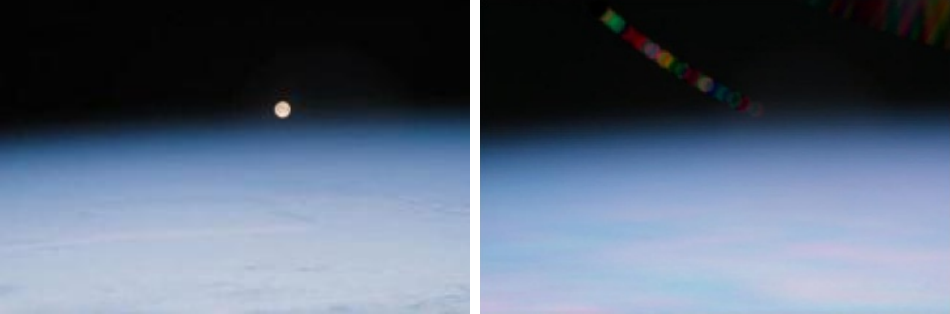
\includegraphics[height=2.1cm]{figures/related/nasa.png}
  \caption{NASA dataset}
  \label{fig:aan_samples_nasa}
\end{subfigure}
\caption[ANN Frame Prediction]{Single frame predictions using an ANN model with two hidden layers.\\
Left: ground truth target frame. Right: generated prediction. (From \parencite{ann})}
\label{fig:aan_samples}
\end{figure}

The loss during the training process was measured in terms of the MS-SSIM index in order to optimize the network to preserve the luminance, constrast and structure of the image. Since the data of the used Fighter and NASA datasets have a high image size, applyting the multi-scale version of SSIM was a reasonable choice.

When we take a look at the presented prediction results of Figure \ref{fig:aan_samples}, it can be seen that the network more or less averages over the input sequence. This effect is clearly visible in Figure \ref{fig:aan_samples_nasa}, were the movement of the moon from the top left towards the earth's horizon is predicted as a like composed of previous moon positions. As a result, this simple architecture does not sufficiently capture the temporal correlations of the input data.

\section{Recurrent Network Approaches}

In order to leverage the sequential structure and temporal correlations of video data, severals works performed frame prediction based on recurrent network models. These following models have inspired our overall model architecutre the most.

\subsection{LSTM Autoencoder Model}

A huge step forward has been taken when the recurrent encoder-decoder framework, earlier presented in Section \ref{sec:rnn_enc_dec}, has been applied in \parencite{unsup_learn_lstm} to perform unsupervised learning of video representations. The fact that the same operation must be applied at each time step to produce the next state was their key idea to use this framework in that context. 

All in all, a LSTM autoencoder model has been presented that was trained to reconstruct an entire input sequence of about ten image frames, similar to Figure \ref{fig:rnn-autoencoder}. This model has been slightly modified in a second step to predict the future sequence of frames. In a last step, both models have been combined to a model that exhibits a single encoder to learn the dynamics of the video, but two different encoders. Initialized by the identical learned representation, the one decoder tries to reconstruct the inputs backward in time, while the other decoder predicts the future frames forward in time. Consequently, the decoder has to come up with a represention that be handled by both decoders. In this way, they tried to compensate the shortcomings of each model, such as the potential tendency of reconstruction decoder to learn the trivial function, or to counteract that the future predictor considers the last frames of the input sequence only. This combined model delivered the best results and is shown in Figure \ref{fig:lstm_combo}.

\begin{figure}[htb]
	\centering
	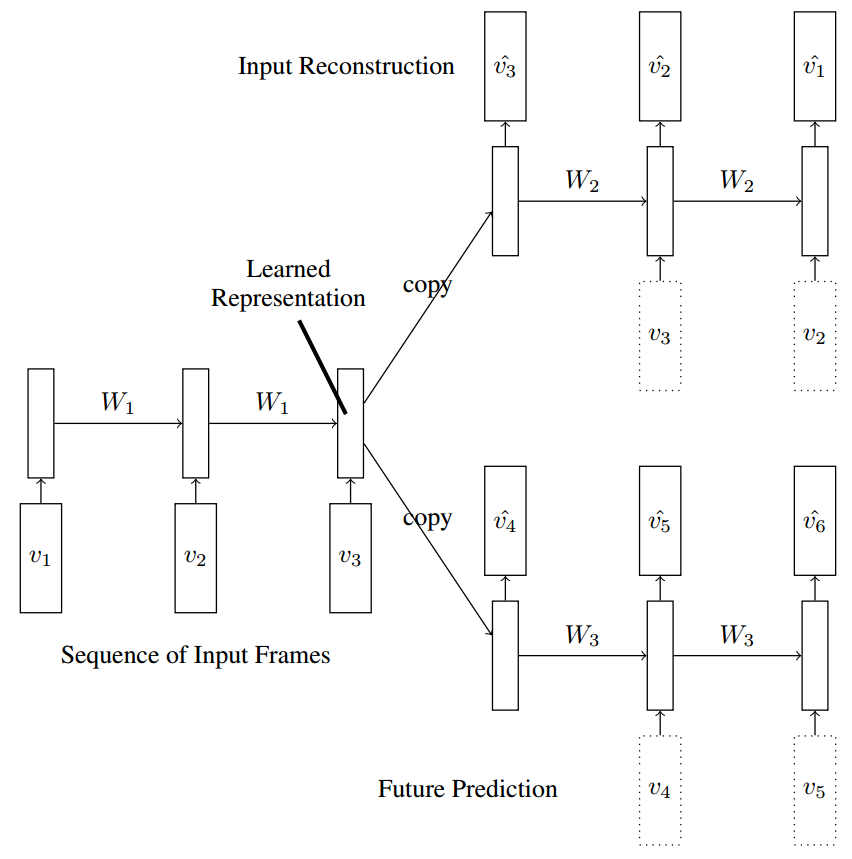
\includegraphics[width=0.5\linewidth]{figures/related/combo_shrinked.png} 
	\caption[Composite LSTM Autoencoder Model]{The composite LSTM autoencoder model. The top branch reconstructs the input sequence backwards in time, while the bottom branch performs frame predictions forward in time.} \label{fig:lstm_combo}
\end{figure}

Within their work, they also explored if the decoder should condition on the previously generated outout or not, as earlier discussed in Section \ref{sec:rnn_enc_dec}. The eventual choice has fallen on the conditioned variant, because it delivered slightly sharper frame predictions in the qualitative evaluation. Besides that, they also varied the number of recurrent layers with the clear result that a deeper LSTM yields best performance.

Another contribution of this work has been the introduction of a simple dataset that can be generated on-the-fly in order to explore the architecture of the model, as well as the effects of hyperparameter changes. It uses handwritten numbers that bounce around in a short sequence of images. Since this dataset has been used in several other subsequent works as well, it offers the ability to be used as a basic benchmark to compare the performance of various models. The dataset will be presented in detail in Section \ref{sec:ds_mm}. Sequences from these and another dataset have then been used as input to the LSTM encoder to train the model. It is to highlight, that they used the full image patch for this purpose. They mentioned to use convolutional percepts of the image sequence as inputs as well, but actually used this approach in the seconds part of their paper only, where they transfered the pre-trained encoder to improve the performance of supervised human action classification in videos.

The authors also pointed out that the choice of the loss function is fundamental with respect to quality of results. Nevertheless, they descided to rely on standard error functions and kept the use of more advanced objective functions for furhter research. To be more precise, they trained their network using binary cross-entropy when applied to MovingMNIST, and squared error for real world tests on UCF-101. Details about the latter dataset can be found in Section \ref{sec:ds_ucf}.

All in all, the strength of this model regarding future frame prediction is that it is able to infer a variable number of frames by taking the temporal correlations of the entire input sequence into account. But as a downside, the use of FC-LSTM cells with such high dimensional inputs implies a huge model complexity in the order of $10^8$ in case of a two-layer LSTM with \num{2048} hidden units each. Consequently, such a model takes a very long time to learn and does not consider spatial properties of each single input, due to the use of fully-connected state transitions.


\subsection{Convolutional LSTM Encoding-Forcasting Model}


\begin{figure}[htb]
	\centering
	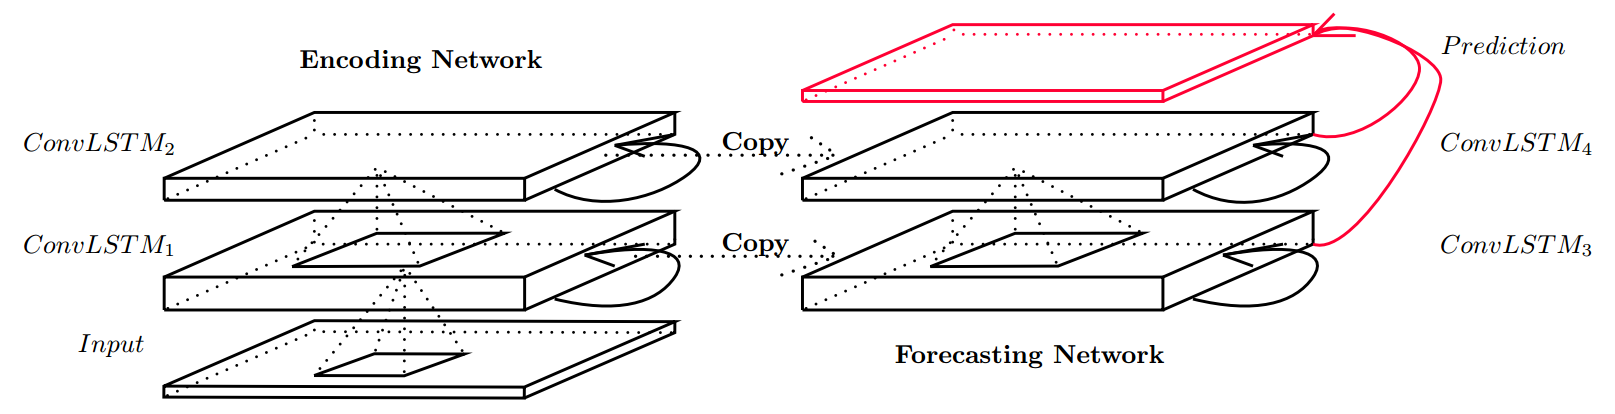
\includegraphics[width=0.8\linewidth]{figures/related/nowcasting_model.png} 
	\caption[Short]{Description.} \label{fig:convlstm_model}
\end{figure}

\subsection{Spatio-Temporal Video Autoencoder Model}

\begin{figure}[htb]
	\centering
	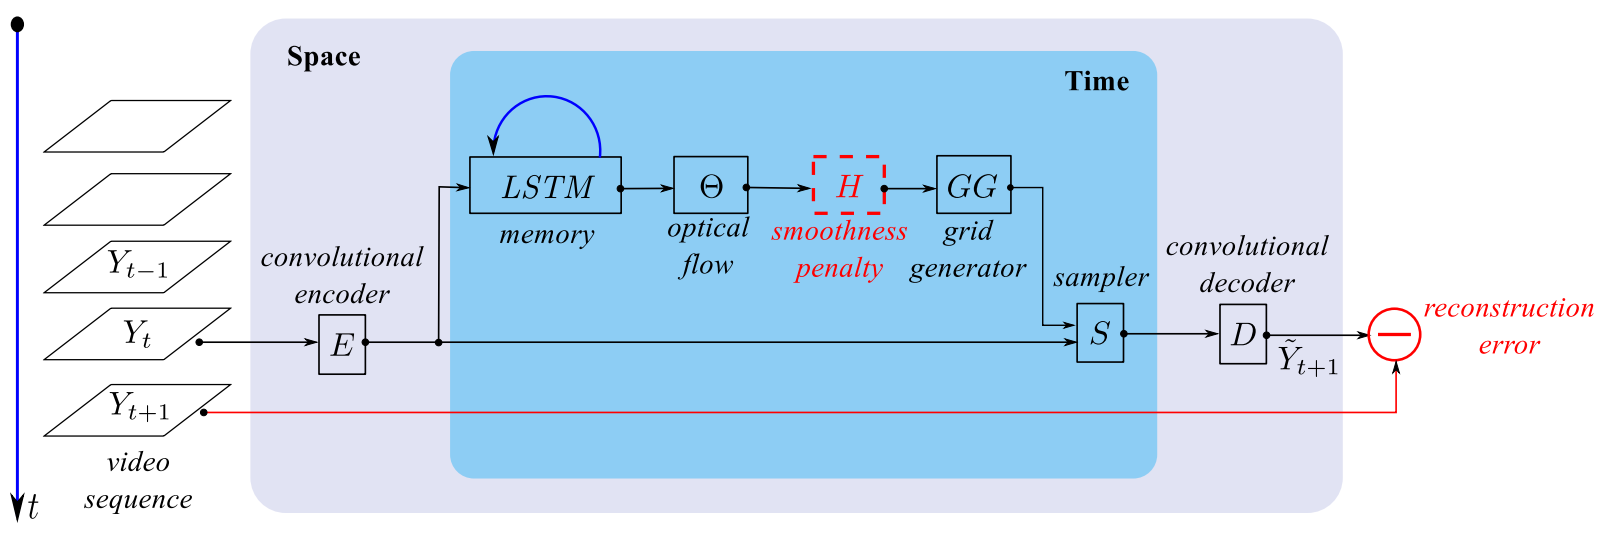
\includegraphics[width=0.8\linewidth]{figures/related/spat_temp_video.png} 
	\caption[Short]{Description.} \label{fig:spatiotemp_model}
\end{figure}


\begin{figure}[htb]
	\centering
	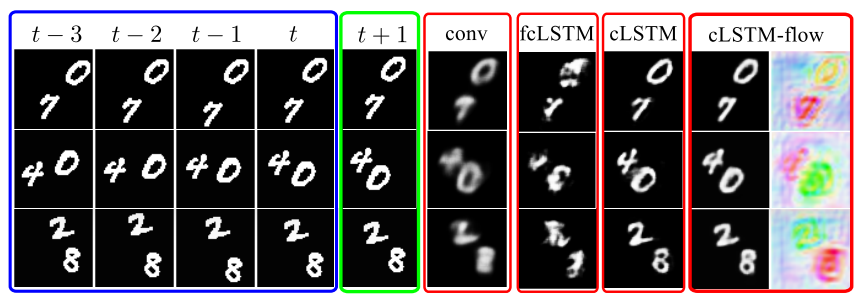
\includegraphics[width=1.0\linewidth]{figures/related/spat_temp_results.png} 
	\caption[Short]{Description.} \label{fig:spatiotemp_results}
\end{figure}


\section{Adversarial Network Approach}


\begin{figure}[htb]
	\centering
	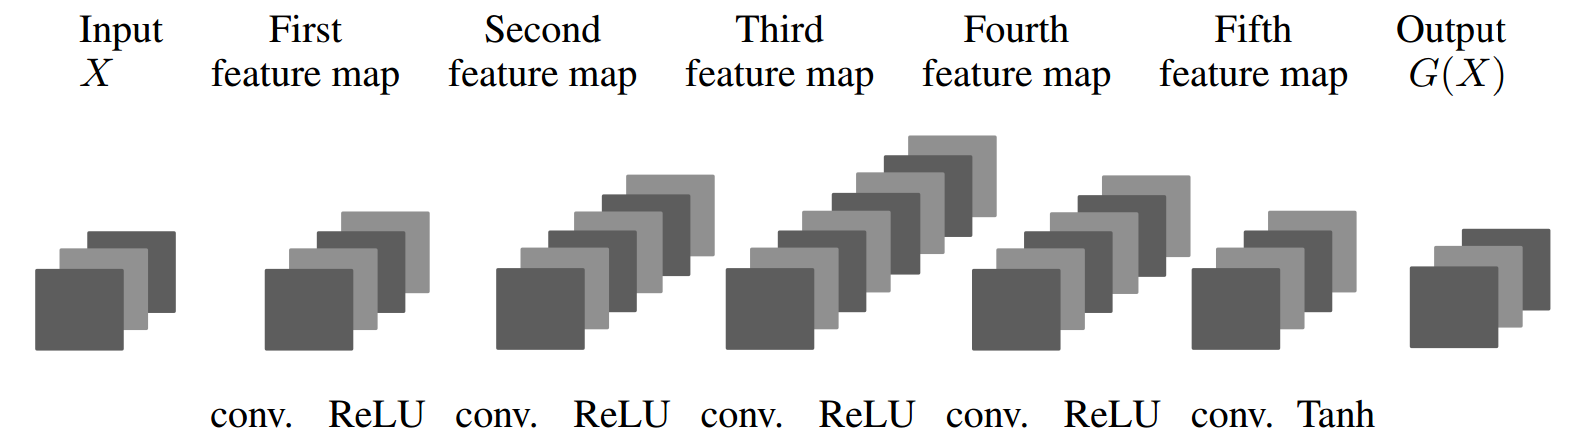
\includegraphics[width=0.8\linewidth]{figures/related/deep_multiscale_generator.png} 
	\caption[Short]{Description.} \label{fig:gan_generator}
\end{figure}


\begin{figure}[htb]
	\centering
	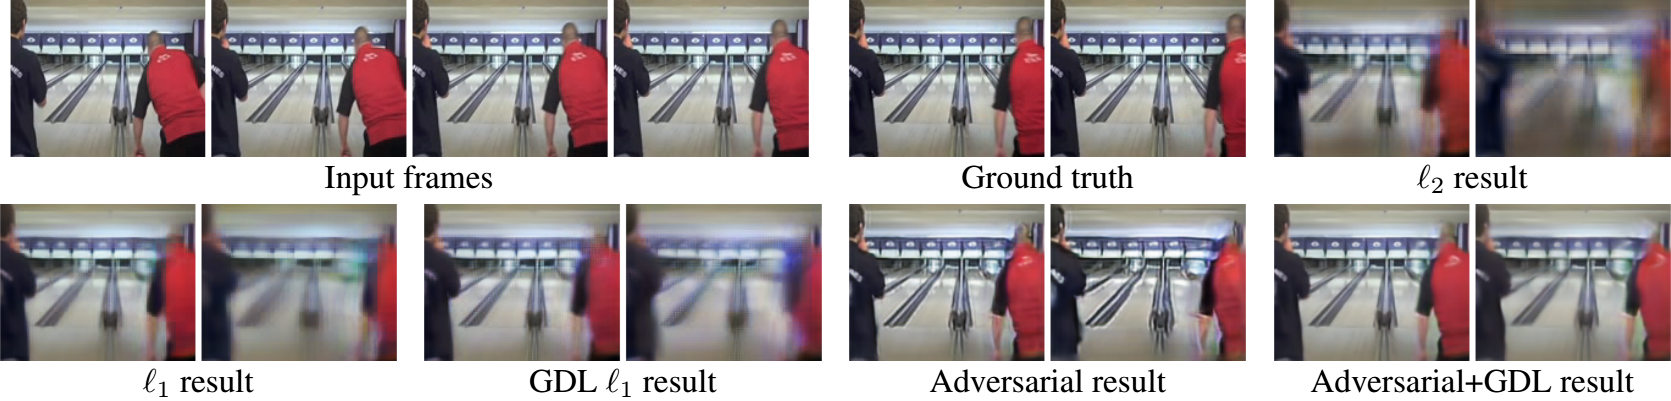
\includegraphics[width=1.0\linewidth]{figures/related/deep_multiscale_samples.png} 
	\caption[Short]{Description.} \label{fig:gan_samples}
\end{figure}





%In \textbf{Chapter \ref{chapter:relatedwork}}, we take a closer look at existing approaches that are suitable for spatio-temporal learning and frame prediction. We briefly discuss their strength and weaknesses, as well as how they have influenced the design decisions regarding the architecture of our final neural network model. Additionally, these presented models build the baselines in our evaluation.